\chapter{Examples}

\section{...for lists}\label{sec:Liste}

\subsection{bullet list}
\begin{itemize}
 \item Frictional resistance $R_F$
 \item viskous resistance $R_{VD}$
 \item Wave resistance $R_W$
\end{itemize}

\subsection{numerated list}

\begin{enumerate}
 \item Frictional resistance $R_F$
 \item Viskous resistance $R_{VD}$
 \item Wave resistance $R_W$
\end{enumerate}

\section{...for a table}
 \begin{table}[h!]
\caption[\textit{Alianca Bahia}'s ship data]{\textit{Alianca Bahia}'s ship data}
\centering
\begin{tabular}{l r c}
 \toprule
    $L_{oa}$ & length over all & $201,04\,m$ \\
    $L_{pp}$ & length between perpendiculars & $189,60\,m$ \\
    $B$ & breadth & $29,80\,m$ \\
    $D$& side height & $16,50\,m$ \\
    $T_d$ & design draught & $10,10\,m$ \\
\bottomrule 
\end{tabular}
\label{tab:shipData}
\end{table}

\section{...for equations}
\subsection{single line}
\begin{equation}
 \Delta=\rho\cdot\nabla \label{equ:T}
\end{equation}

\subsection{multi line}
\begin{eqnarray}
 g\cdot\Delta=&g\cdot\rho\cdot\nabla\\
 G =& B \label{equ:delta}
\end{eqnarray}
\clearpage


\section{...for figures}\label{sec:tables}

\subsection{single picture}
\begin{figure}[t]
\centering
  \includegraphics[width=0.8\textwidth]{./figures/bugwulst_abmessungen2.pdf}
  \caption[Bulbuos bow parameter]{Bulbuos bow parameters, figure as in \cite{Kracht}}\label{fig:bulbuosBowKracht}
\end{figure}

In equation \eqref{equ:delta}

\subsection{Multiple pictures}

\begin{figure}[ht]
    \centering
    \begin{subfigure}[ht]{.45\textwidth}
        \includegraphics[width=\textwidth]{./figures/bug.png}  
        \caption{Bow view}
        \label{fig:sub-bow}
    \end{subfigure}
    \hfill
    \begin{subfigure}[ht]{.45\textwidth}
        \includegraphics[width=\textwidth]{./figures/heck.png}  
        \caption{Stern view}
        \label{fig:sub-stern}
    \end{subfigure}
    \caption[CFD result]{CFD-result of a $14\,000\;TEU$ container ship}
    \label{fig:CFD}
\end{figure}

\clearpage

\section{...for plots}
\subsection{plotting with direct coordinates}

\begin{figure}[h!]
  \begin{center}
		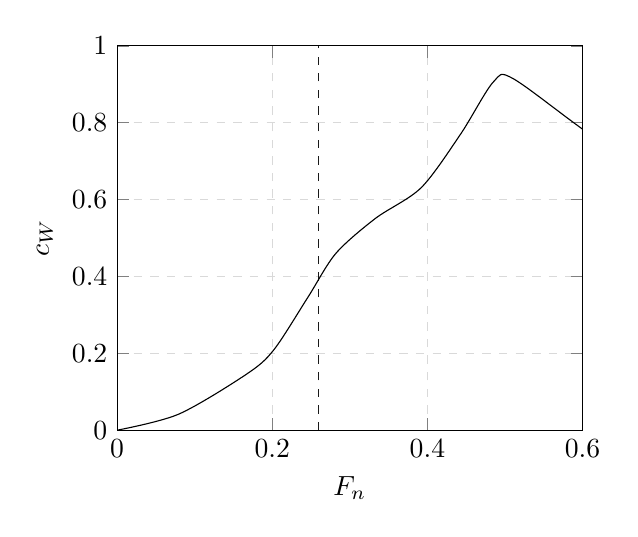
\begin{tikzpicture}
		\begin{axis}[
		width=0.618\textwidth,
		grid=major,
		grid style={dashed,gray!30},
		xmin=0,xmax=0.6,
		ymin=0,ymax=1,
		xlabel=$F_n$,
		ylabel=$c_W$,]
		\addplot[smooth,color=black]
			coordinates {(0,0)(0.0794,0.0417)(0.167,0.146)(0.202,0.209)(0.246,0.346)(0.282,0.46)(0.333,0.551)(0.392,0.631)(0.443,0.771)(0.485,0.906)(0.511,0.914)(0.618,0.758)(0.733,0.623)(0.872,0.496)};
	\addplot [color=black, dashed, opacity=0.9]coordinates{(0.26,0)(0.26,1)};
		\end{axis}
		\end{tikzpicture}
    \caption{Wave resistance over froude number according to \cite{jensen}}\label{fig:cwfroude}
  \end{center}
\end{figure}

\subsection{plotting a mathematical function}
\begin{figure}
    \centering
    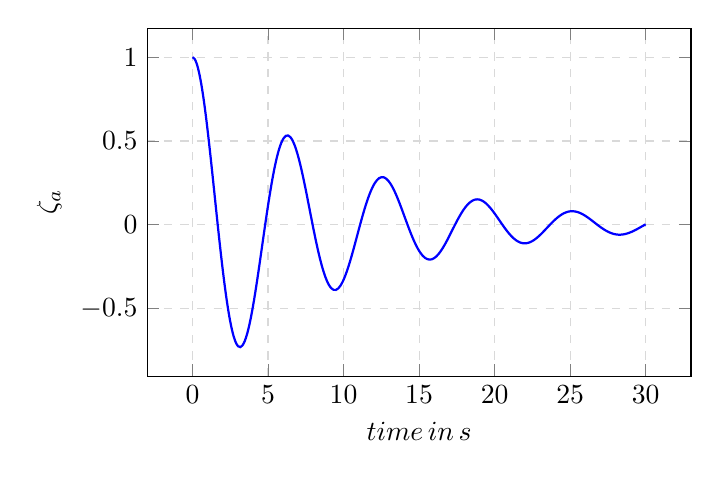
\begin{tikzpicture}
    \begin{axis}[
          width=0.7\textwidth,
          height=6cm,
          grid=major, 
          grid style={dashed,gray!30},
          xlabel= $time \, in \,  s$,
          ylabel= $\zeta_a$]
        \addplot[
            domain = 0:30,
            samples = 200,
            smooth,
            thick,
            blue,
        ] {exp(-x/10)*( cos(deg(x)) + sin(deg(x))/10 )};
    \end{axis}
    \end{tikzpicture}
    \caption{Plotting a mathematical function directly in latex}
    \label{fig:plotFunc}
\end{figure}

\clearpage

\subsection{plotting .csv table data}
\begin{figure}[h!]
  \begin{center}
    \begin{tikzpicture}
      \begin{axis}[
          width=0.7\textwidth,
          grid=major, 
          grid style={dashed,gray!30},
          xlabel= $Optimierungsschritt$,
          ylabel= $c_T$]
        \addplot [mark=*, color=darkblue, opacity=0.8, mark size=0.8, only marks]
        table[x=Anz,y=eval_CT,col sep=comma] {./tables/dataTable.csv};      
      \end{axis}
    \end{tikzpicture}
    \caption[Plot from .csv file]{Plotting a graph from a table brings the advantage, that with chaged data, only the new file has to be exported and after the next compilation, every figure is up to date.}\label{fig:tableplot}
  \end{center}
\end{figure}
\clearpage

\section{...for referencing and citing}
\subsection{referencing}
e.g.:\\
Refer section \ref{sec:Liste}\\
In table \ref{tab:shipData}...\\
Equation \ref{equ:T} and \ref{equ:delta}....\\
Die Grafik \ref{fig:sub-bow} in Abbildung \ref{fig:CFD}....

\subsection{citing literature}
In \cite{Schiffstechnik} fundamental basics of naval architecture can be found.

Figure \ref{fig:bulbuosBowKracht} shows a slightly modified picture as found in \cite{Kracht}.

\section{...for writing code in \LaTeX}


\begin{lstlisting}[caption={A simple code example}]
for (int i=0; i<5;i++)
{
    do something;
}
\end{lstlisting}

\chapter{Off you go!}

Now after some examples, it's up to you to fill these pages with life.  